\documentclass[11pt,a4paper,oneside]{report}
% Preamble of the pyBones report. Built with XeLaTeX (latexmk, see latexmkrc).
% Formal layout: Latin Modern fonts, black headings, colour only where it carries meaning.

\usepackage[a4paper,top=2.5cm,bottom=2.5cm,left=2.5cm,right=2.5cm,headheight=14pt]{geometry}
\usepackage{fontspec}   % Latin Modern (default), Unicode input
\usepackage{microtype}

% ---------------------------------------------------------------- colours
\usepackage{xcolor}
\definecolor{accent}{HTML}{1F3A68}      % links, plot annotations (dark blue)
\definecolor{ink}{HTML}{000000}
\definecolor{muted}{HTML}{555555}
\definecolor{boneC}{RGB}{80,200,80}     % label colours of pybones (render.colors_bgr)
\definecolor{vesselC}{RGB}{230,40,40}
\definecolor{burstC}{RGB}{40,150,230}
\definecolor{legacyC}{HTML}{9A9A9A}

% ---------------------------------------------------------------- packages
\usepackage{amsmath}
\usepackage{graphicx}
\graphicspath{{figures/}{2018/images/}}
\usepackage{booktabs}
\usepackage{tabularx}
\usepackage{enumitem}
\setlist{itemsep=2pt,topsep=4pt}
\usepackage[font=small,labelfont=bf,labelsep=period]{caption}
\usepackage{subcaption}
\usepackage{tikz}
\usetikzlibrary{arrows.meta,positioning}
\usepackage{pgfplots}
\usepackage{pgfplotstable}
\pgfplotsset{compat=1.18}
\usepackage{xurl}
\usepackage[colorlinks=true,linkcolor=accent,urlcolor=accent,citecolor=accent]{hyperref}

% ---------------------------------------------------------------- headings and page style
\usepackage{titlesec}
\titleformat{\chapter}[hang]{\Huge\bfseries}{\thechapter}{0.6em}{}
\titlespacing*{\chapter}{0pt}{0pt}{20pt}
\titleformat{\paragraph}[runin]{\normalfont\bfseries}{}{0pt}{}[.]

\usepackage{fancyhdr}
\pagestyle{fancy}
\fancyhf{}
\fancyhead[L]{\small\nouppercase{\leftmark}}
\fancyhead[R]{\small\thepage}
\renewcommand{\headrulewidth}{0.4pt}
\fancypagestyle{plain}{\fancyhf{}\fancyfoot[C]{\small\thepage}\renewcommand{\headrulewidth}{0pt}}

% ---------------------------------------------------------------- macros
\newcommand{\um}{\,\ensuremath{\mu}m}                 % micrometres
\newcommand{\umsq}{\,\ensuremath{\mu}m\ensuremath{^2}}
\newcommand{\umcube}{\,\ensuremath{\mu}m\ensuremath{^3}}
\newcommand{\code}[1]{\texttt{#1}}
\newcommand{\lbl}[2]{\textcolor{#1}{\textbf{#2}}}     % a label name, in its overlay colour
\newcommand{\bone}{\lbl{boneC}{bone}}
\newcommand{\vessel}{\lbl{vesselC}{vessel}}
\newcommand{\burst}{\lbl{burstC}{burst}}

% A framed remark.
\newsavebox{\keybox}
\newenvironment{keypoint}
  {\par\medskip\noindent\begin{lrbox}{\keybox}%
   \begin{minipage}{\dimexpr\linewidth-2\fboxsep-2\fboxrule\relax}\small}
  {\end{minipage}\end{lrbox}\fbox{\usebox{\keybox}}\par\medskip}

% One captioned image panel of a figure row: \panel{fraction of the line width}{file}{caption}
\newcommand{\panel}[3]{\begin{subfigure}[t]{#1\linewidth}\centering
  \includegraphics[width=\linewidth]{#2}\caption{#3}\end{subfigure}}

% Generated by tools/report (values measured on the data, never typed by hand).
\newcommand{\pbValueThrBone}{9{,}382}
\newcommand{\pbValueThrVessel}{22{,}652}
\newcommand{\pbValueMeanBackground}{5{,}675}
\newcommand{\pbValueMeanBone}{13{,}064}
\newcommand{\pbValueMeanVessel}{32{,}215}
\newcommand{\pbValueFracBone}{18.7}
\newcommand{\pbValueFracVessel}{2.24}
\newcommand{\pbValueFracBurst}{0.93}
\newcommand{\pbValueSeconds}{24}
\newcommand{\pbValuePeakGB}{1.7}
\newcommand{\pbValueCpu}{AMD Ryzen AI 9 HX 370 w/ Radeon 890M}
\newcommand{\pbValueCores}{24}
\newcommand{\pbValueMemoryGB}{23}
\newcommand{\pbValueSystem}{CachyOS (Linux 7.3.5-2-cachyos)}
\newcommand{\pbValuePython}{3.12.15}
\newcommand{\pbValuePowerProfile}{balanced}
\newcommand{\pbValueStageWeightTolerance}{0.05}
\newcommand{\pbValueWorkers}{4}
\newcommand{\pbValueVersion}{0.7.0}
\newcommand{\pbValueProfileCore}{64{,}244}
\newcommand{\pbValueProfileHalfMax}{34{,}959}
\newcommand{\pbValueBoneDice}{0.989}
\newcommand{\pbValueBonePrecision}{0.994}
\newcommand{\pbValueBoneRecall}{0.984}
\newcommand{\pbValueVesselDice}{0.862}
\newcommand{\pbValueVesselPrecision}{0.826}
\newcommand{\pbValueVesselRecall}{0.901}
\newcommand{\pbValueBurstDice}{0.922}
\newcommand{\pbValueBurstPrecision}{0.904}
\newcommand{\pbValueBurstRecall}{0.940}
\newcommand{\pbValueAccuracy}{0.987}
\newcommand{\pbValueVesselRecallThin}{0.43}
\newcommand{\pbValueVesselRecallMedium}{0.84}
\newcommand{\pbValueVesselRecallLarge}{0.91}
\newcommand{\pbValueClottedRecall}{0.82}
\newcommand{\pbValueMeshBoneTriangles}{6.94}
\newcommand{\pbValueMeshBonePoints}{3.46}
\newcommand{\pbValueMeshBoneSeconds}{13}
\newcommand{\pbValueMeshBoneGlbMB}{124.8}
\newcommand{\pbValueMeshVesselTriangles}{2.72}
\newcommand{\pbValueMeshVesselPoints}{1.36}
\newcommand{\pbValueMeshVesselSeconds}{6}
\newcommand{\pbValueMeshVesselGlbMB}{49.0}
\newcommand{\pbValueMeshBurstTriangles}{0.19}
\newcommand{\pbValueMeshBurstPoints}{0.10}
\newcommand{\pbValueMeshBurstSeconds}{2}
\newcommand{\pbValueMeshBurstGlbMB}{3.5}
\newcommand{\pbValueMeshComparedStlMB}{136.0}
\newcommand{\pbValueMeshComparedGlbFloatMB}{65.4}
\newcommand{\pbValueMeshErrorUm}{0.05}
\newcommand{\pbValueMeshErrorVoxelRatio}{57}
\newcommand{\pbValueMeshGridUm}{6}
\newcommand{\pbValueNetSeconds}{18}
\newcommand{\pbValueNetStackDepthUm}{300}
\newcommand{\pbValueNetBranches}{9{,}514}
\newcommand{\pbValueNetTruncated}{1{,}459}
\newcommand{\pbValueNetJunctions}{3{,}121}
\newcommand{\pbValueNetLoops}{120}
\newcommand{\pbValueNetFreeEnds}{6{,}044}
\newcommand{\pbValueNetFaceEnds}{1{,}836}
\newcommand{\pbValueNetBurstEnds}{298}
\newcommand{\pbValueNetLengthMm}{592}
\newcommand{\pbValueNetDensity}{64.1}
\newcommand{\pbValueNetMedianBranchUm}{37}
\newcommand{\pbValueNetMedianRadiusUm}{6.7}
\newcommand{\pbValueNetMedianTortuosity}{1.13}
\newcommand{\pbValueNetPhantomVessels}{24}
\newcommand{\pbValueNetPhantomDepth}{3}
\newcommand{\pbValueNetTolerance}{6}
\newcommand{\pbValueNetJunctionTolerance}{20}
\newcommand{\pbValueNetAnchorMargin}{3}
\newcommand{\pbValueNetSpurFactor}{2}
\newcommand{\pbValueNetLoopFactor}{1.5}
\newcommand{\pbValueNetTrueForks}{53}
\newcommand{\pbValueNetTrueMaskMissed}{13}
\newcommand{\pbValueNetTrueMaskCycles}{4}
\newcommand{\pbValueNetSegCycles}{7}
\newcommand{\pbValueNetTrueMaskForks}{40}
\newcommand{\pbValueNetTrueMaskSpurious}{8}
\newcommand{\pbValueNetSegForks}{26}
\newcommand{\pbValueNetSegSpurious}{49}
\newcommand{\pbValueNetSegRecall}{0.79}
\newcommand{\pbValueNetSegPrecision}{0.85}
\newcommand{\pbValueNetSegLengthErrorPct}{$-3.0$}
\newcommand{\pbValueNetTrueLengthErrorPct}{$+8.2$}
\newcommand{\pbValueNetSegRadiusOffset}{$-0.82$}
\newcommand{\pbValueNetSegRadiusThin}{$+0.8$}
\newcommand{\pbValueNetSegRadiusThick}{$-1.5$}
\newcommand{\pbValueNetTrueRadiusThick}{$-1.0$}
\newcommand{\pbNumThrBone}{9382}
\newcommand{\pbNumThrVessel}{22652}
\newcommand{\pbNumMeanBackground}{5675}
\newcommand{\pbNumMeanBone}{13064}
\newcommand{\pbNumMeanVessel}{32215}
\newcommand{\pbNumProfileHalfMax}{34959}

\pgfplotstableread[col sep=comma]{data/history.csv}\historytable


\title{pyBones}
\author{Luraminaki}

\begin{document}

% ---------------------------------------------------------------- title page
\begin{titlepage}
  \centering
  \vspace*{3cm}
  {\Huge\bfseries pyBones\par}
  \vspace{0.8cm}
  {\Large Segmentation and 3D modelling of the intra-osseous vascular network\\
    of a mouse knee from micro-computed tomography\par}
  \vspace{0.6cm}
  \rule{0.6\linewidth}{0.4pt}\par
  \vspace{0.6cm}
  {\large From a 2018 student project to a validated pipeline\par}
  \vfill
  {\large Luraminaki\par}
  \vspace{0.3cm}
  {Version \pbValueVersion\par}
  \vspace{2cm}
  {\small Rework of a 2017--2018 engineering student project (CPE Lyon, 5ETI -- IMI major),\\
    carried out for the SAINBIOSE laboratory (U1059, Saint-Étienne).\par}
\end{titlepage}

\pagenumbering{roman}
\tableofcontents
\clearpage
\pagenumbering{arabic}

\chapter{Introduction}

\section{Context}

Bone is irrigated by a dense network of blood vessels, and osteoarthritis is thought to change it.
In 2017, the SAINBIOSE laboratory (U1059, Saint-Étienne) was studying these changes in animal models:
the researchers injected a radio-opaque contrast agent (barium sulfate) into the circulation of mice,
then imaged the knee by micro-computed tomography ($\mu$CT, GE Nanotom). The barium makes the vessels
visible to X-rays, but no software was dedicated to measuring a \emph{vascular} network inside bone:
the tools they had were made for bone histomorphometry.

The laboratory proposed the problem as a final-year project at CPE Lyon (5ETI -- IMI major,
2017--2018), and I was one of the four students who took it on. The brief was to separate the vascular
network from the bone tissue, reconstruct it in 3D and, in the longer run, quantify it (number of nodes
and branches, vessel calibre, branch lengths). In a few weeks we delivered a Matlab segmentation and a
Python viewer, which the researchers approved. Chapter~\ref{chap:legacy} summarises what we did.

Looking back at it eight years later, I find our approach naive: every parameter was a pixel count tuned
by eye on a single scan, and nothing told us whether a change made the segmentation better or worse.
I wanted to know how far the same problem could be taken with a clean method, so I rewrote the project
from scratch. This report covers that rewrite, \textbf{pyBones}. I set myself four goals at the start:
\begin{itemize}
  \item no Matlab: Python only, with a minimal set of dependencies (numpy and OpenCV for the
        computations, pydantic for the configuration, scikit-image for marching cubes only; later,
        FastAPI and uvicorn for the web server, three.js, kept in the repository, for the page, and
        scikit-image's 3D skeletonisation and SciPy for the vascular quantification);
  \item clean, documented, tested code, every tunable value in a validated configuration file;
  \item computation speed and memory as first-class concerns, but correctness first;
  \item improve the results, and \emph{prove} it.
\end{itemize}

\section{The data}

The only dataset I have is a stack of 100 slices of a mouse knee: the distal femur on top, the proximal tibia
below, the joint and menisci in between (Figure~\ref{fig:overview-raw}). Each slice is a
$2300 \times 1487$ 16-bit image; the stack weighs about 685\,MB. The 2018 project used a slice
thickness of 3\um; I assumed isotropic 3\um{} voxels, which gives anatomically consistent sizes
(a knee about 3\,mm wide, a femoral cortex about 165\um{} thick).

Three kinds of material appear, from dark to bright:
\begin{itemize}
  \item soft tissue and marrow (background), mean intensity \pbValueMeanBackground;
  \item \bone{} (cortex and trabeculae), mean \pbValueMeanBone;
  \item barium-filled vessels, mean \pbValueMeanVessel, and much brighter clusters where the contrast
        agent leaked out of vessels. The researchers had told us that the knee went through a freezer:
        ice can rupture vessels, and blood can clot inside them. The leaked clusters are labelled
        \burst{}; clotted vessels appear as dim, partially filled \vessel{} segments.
\end{itemize}

\begin{figure}[ht]
  \centering
  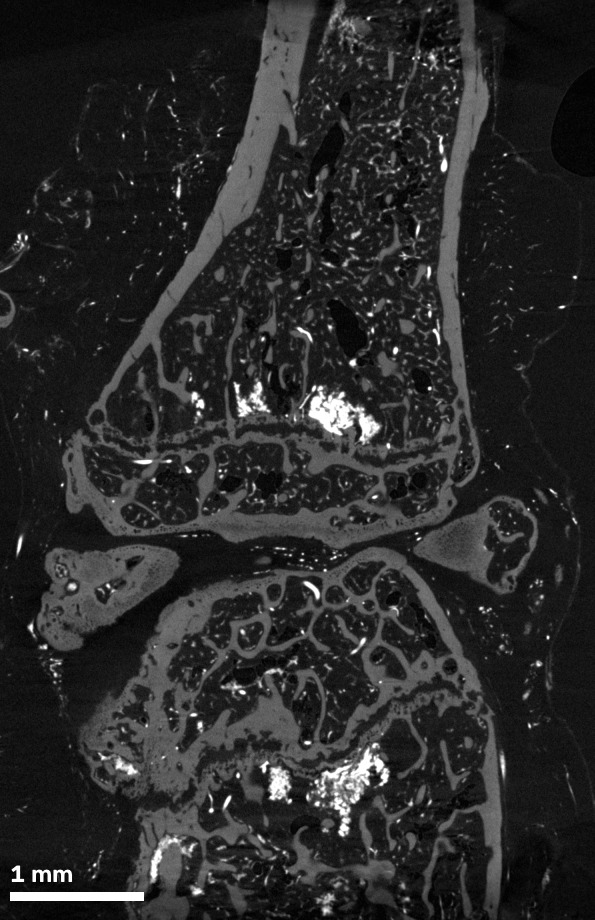
\includegraphics[width=0.48\linewidth]{overview_raw.jpg}
  \caption{Slice 0 of the stack (contrast-stretched). Femur on top, tibia below. The bright white
    clusters inside the bone are bursts of contrast agent; the bright threads are vessels.}
  \label{fig:overview-raw}
\end{figure}

\section{Structure of this report}

Chapter~\ref{chap:legacy} summarises the 2018 project and its limitations. Chapter~\ref{chap:rewrite}
presents the architecture of the rewrite, its web server and the page that replaces our 2018 viewer. Chapter~\ref{chap:segmentation} explains each step of the
segmentation, why I built it that way, and what it changed. Chapter~\ref{chap:validation} shows how I
validated the results without any expert annotation, and how every intermediate version of the
rewrite scores on the same synthetic ground truth. Chapter~\ref{chap:performance} covers speed and
memory, Chapter~\ref{chap:limitations} what is still out of reach, and Chapter~\ref{chap:conclusion}
concludes. Appendix~\ref{chap:reproduce} lists the commands that reproduce every figure and number.

\begin{keypoint}
Every measured value quoted in this report (thresholds, scores, timings, and the machine they were
measured on) is generated by \code{python -m tools.report} from the data and the git history; none
of them is typed by hand.
\end{keypoint}

\chapter{The 2018 project}
\label{chap:legacy}

In 2018 we built two things: a segmentation of the slices in Matlab, and a Python application that
turned its masks into a 3D model. This chapter summarises both, then looks back at their limitations.
The masks our segmentation produced on the reference stack serve as the 2018 baseline in the rest of
this report.

\section{The brief}

The laboratory's brief listed six goals: be compatible with the laboratory's tools (Windows, ImageJ,
CTan); threshold the vascular network apart from the bone; reconstruct and improve the continuity of
the network; build the tools needed to quantify it (nodes, branches, vessel size, branch length);
study the inter- and intra-sample reproducibility; automate the measurements.

\section{Segmentation (Matlab)}

We weighed machine learning against mathematical morphology. Machine learning could learn subjective
criteria, but needed a large labelled database that the researchers would have had to build;
morphology was quick to set up and gave immediate results. We chose morphology, developed in Matlab,
in three versions.

\paragraph{Version 1: thresholds} The 16-bit histogram shows distinct modes
(Figure~\ref{fig:legacy-histogram}). A two-level Otsu threshold (\code{multithresh}), computed
\emph{for each slice}, split the image into background, bone and bright contrast agent. The bone and
the burst clusters were cleanly separated, but many vessels were still counted as bone.

\paragraph{Version 2: openings and closings} Connected components larger than 700 pixels were
declared bone; smaller foreground blobs became ``dark'' vessels. Burst clusters were searched among the
bright pixels: dilated bright regions larger than 1000 pixels with a squarish bounding box, plus dark
regions found by adaptive binarisation and kept if their intensity standard deviation exceeded 2500,
then closed, dilated and reconstructed with disks of 5 to 15 pixels. The researchers approved this
segmentation, while acknowledging ``zones of uncertainty'' between vessels and trabeculae.

\paragraph{Version 3: slice-to-slice connectivity} Each slice was corrected with its two neighbours,
a three-slice majority vote: a pixel set in slices $n-1$ and $n+1$ but not in $n$ was added
($101 \rightarrow 111$), an isolated one removed ($010 \rightarrow 000$). The masks of bone and
vessels were written as PNG images, one pair per slice; bursts were discarded.

\begin{figure}[ht]
  \centering
  \begin{subfigure}[t]{0.32\linewidth}\centering
    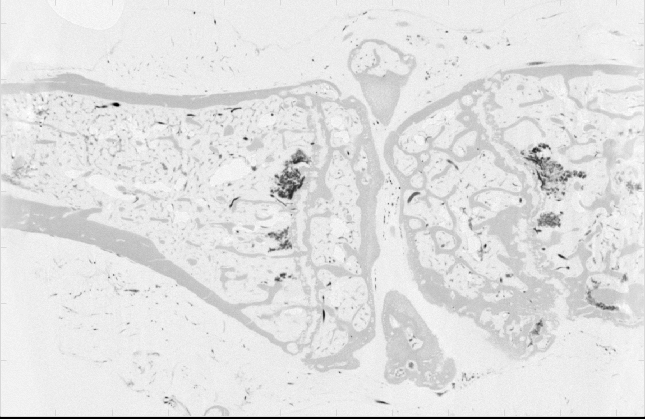
\includegraphics[angle=-90,width=\linewidth]{original.png}\caption{Original slice.}
  \end{subfigure}\hfill
  \begin{subfigure}[t]{0.32\linewidth}\centering
    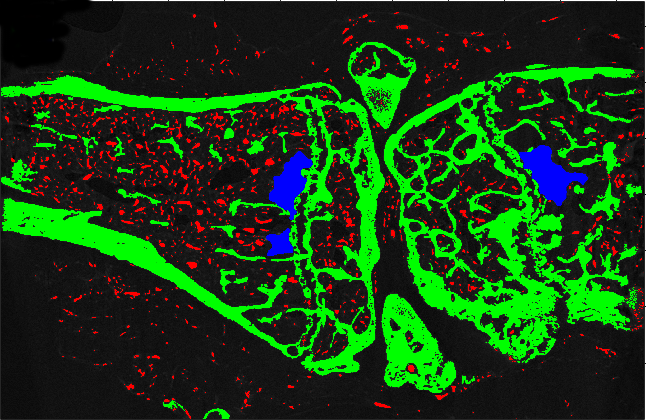
\includegraphics[angle=-90,width=\linewidth]{results2.png}\caption{Version 2.}
  \end{subfigure}\hfill
  \begin{subfigure}[t]{0.32\linewidth}\centering
    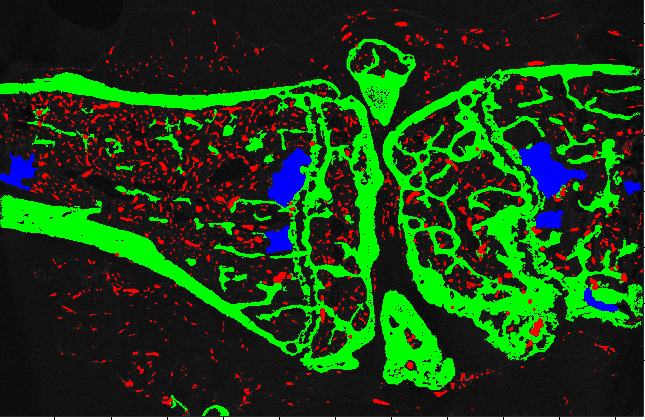
\includegraphics[angle=-90,width=\linewidth]{results3.png}\caption{Version 3.}
  \end{subfigure}
  \caption{Our 2018 segmentation, in the colours we used then: bone in green, vessels in red, burst
    clusters in blue.}
  \label{fig:legacy-results}
\end{figure}

\begin{figure}[ht]
  \centering
  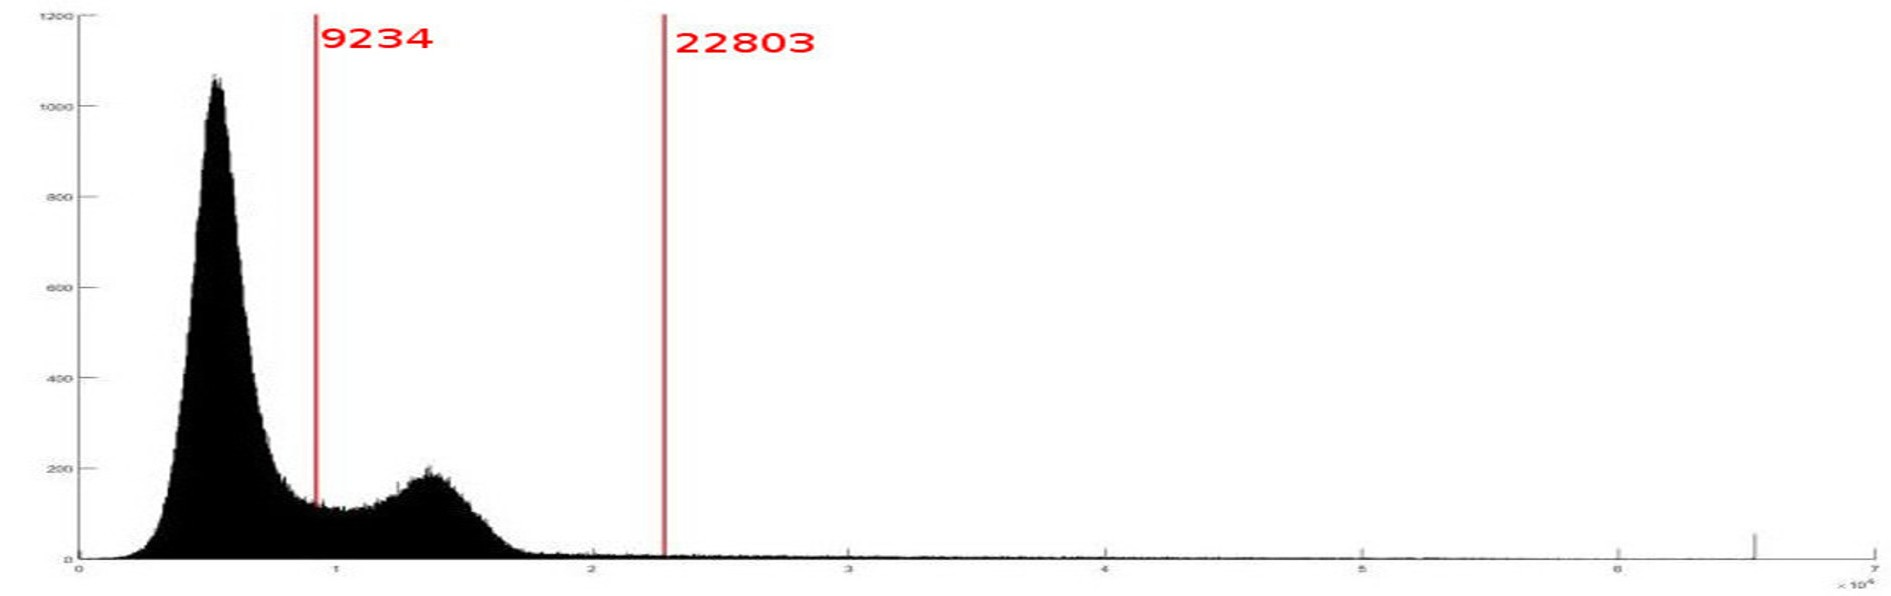
\includegraphics[width=0.7\linewidth]{histogrammeshort.jpg}
  \caption{Histogram of one slice (2018 figure): its modes motivated the multi-level threshold.}
  \label{fig:legacy-histogram}
\end{figure}

\section{3D modelling (Python, PyQt5)}

The second half of the project turned the masks into a 3D model. Our PyQt5 application let the user pick
a folder of masks, enter the physical dimensions and a ``marching cube accuracy'' between 1 and 50
(the step of the algorithm), then: stack the PNG masks into a Matlab \code{.mat} volume; run the
Lewiner marching cubes of scikit-image; either display the mesh with matplotlib's
\code{Poly3DCollection}, or save it as an STL file, checked on an online viewer
(Figure~\ref{fig:legacy-modelling}). We had already noted at the time that the matplotlib rendering was
slow, memory-hungry and badly scaled, that the STL showed the ``cubic aspect'' of marching cubes, and
that the program needed a lot of memory. Chapter~\ref{chap:rewrite} describes what replaces it today:
a web page drawing smoothed meshes on the graphics card.

\begin{figure}[ht]
  \centering
  \begin{subfigure}[t]{0.32\linewidth}\centering
    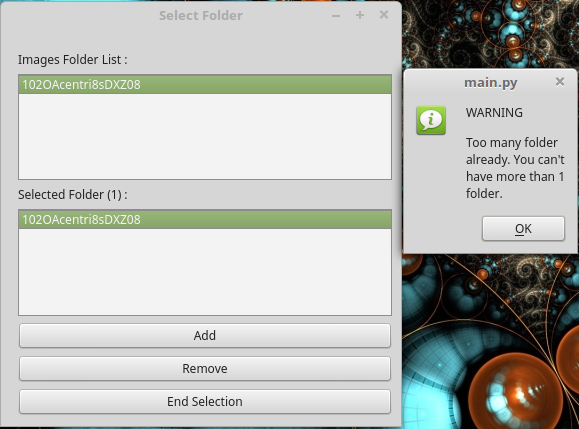
\includegraphics[height=4cm,width=\linewidth,keepaspectratio]{IHM02.png}
    \caption{PyQt5 interface.}
  \end{subfigure}\hfill
  \begin{subfigure}[t]{0.32\linewidth}\centering
    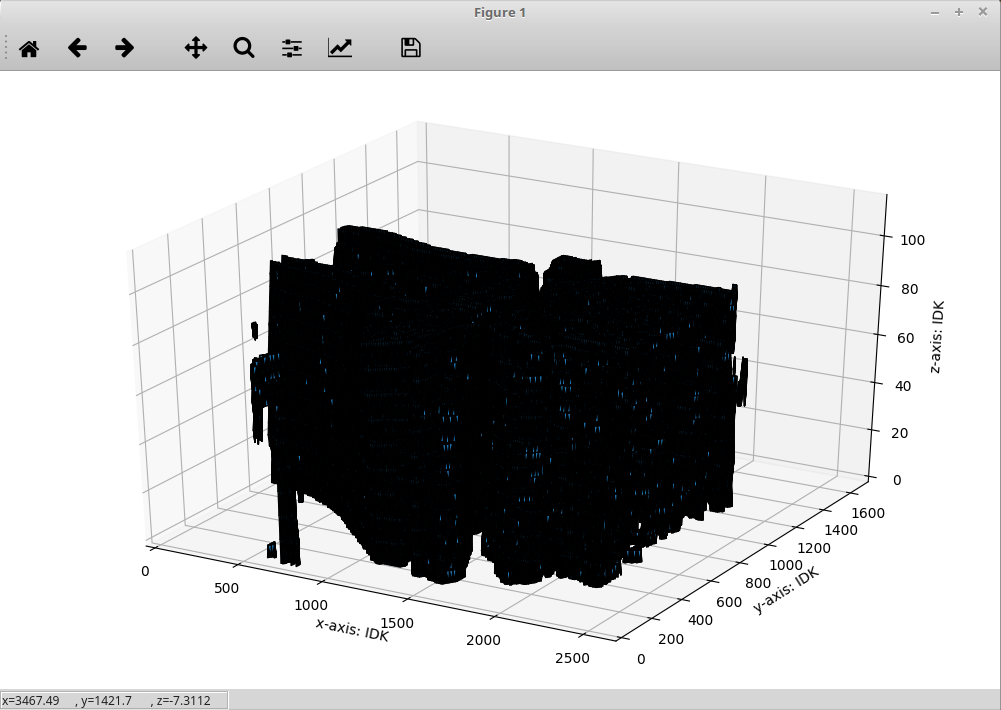
\includegraphics[height=4cm,width=\linewidth,keepaspectratio]{Plot3D01.png}
    \caption{Matplotlib rendering.}
  \end{subfigure}\hfill
  \begin{subfigure}[t]{0.32\linewidth}\centering
    \raisebox{\depth}{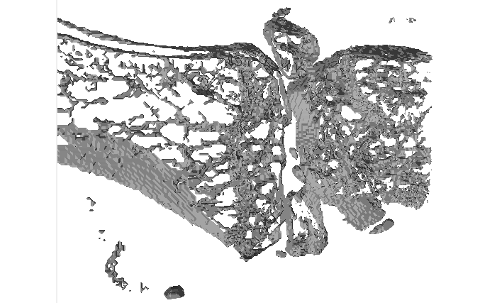
\includegraphics[angle=-90,totalheight=4cm,width=\linewidth,keepaspectratio]{STL01.png}}
    \caption{STL in a viewer.}
  \end{subfigure}
  \caption{The 2018 modelling application.}
  \label{fig:legacy-modelling}
\end{figure}

\section{Limitations}

Looking back with the data at hand, our project had the merit of working end to end in a few weeks,
and of identifying the real difficulty (vessels versus trabeculae). Its limitations fall into three
groups.

\paragraph{Method}
\begin{itemize}
  \item \textbf{Hand-tuned pixel counts.} We tuned every parameter (700 pixels, disks of 5 to 15
        pixels, a standard deviation of 2500 grey levels) on this scan, in pixels. At another
        resolution, or on another animal, none of them keeps its meaning.
  \item \textbf{Per-slice thresholds.} Each slice got its own Otsu thresholds, so the same tissue
        could change class from one slice to the next.
  \item \textbf{Vessel size.} The vessel masks are much thicker than the vessels: their boundary was
        set by morphology, not by the physics of the image (Section~\ref{sec:edges} measures it).
  \item \textbf{Ambiguous blobs.} Every small bone-intensity blob became a vessel. Some are
        dim (clotted) vessels, others are cross-sections of trabecular rods: a 2D slice cannot tell.
  \item \textbf{Bursts discarded} rather than delineated, and \textbf{thin structures eroded} by the
        three-slice vote, which deletes anything only one slice thick.
\end{itemize}

\paragraph{Engineering} The pipeline needed Matlab, exchanged hundreds of intermediate PNG and
\code{.mat} files, hard-coded its paths, held whole volumes in memory, and had no tests.

\paragraph{Validation} Apart from the researchers' visual approval, nothing measured the quality of the
segmentation, so we could not show that any change was an improvement. We did not reach the
quantification goals of the brief.

\chapter{The rewrite}
\label{chap:rewrite}

\section{Principles}

\paragraph{Physical, not pixel, parameters} The first rule I set was to state every length, area and
volume of the configuration in physical units. They are expressed in \um, \umsq{} or \umcube, and converted to pixels once, from the voxel size
(\code{acquisition.}\allowbreak\code{voxel\_size\_um}). Anisotropic voxels are supported: in-plane kernels become
ellipses, 3D neighbourhoods become balls made of per-slice ellipses. Changing the resolution, or
scanning another species, means stating anatomically meaningful sizes, not re-tuning pixel counts.
I build the kernels analytically: OpenCV's elliptic structuring elements carry one-pixel spikes at
their tips, and a one-row ``ellipse'' degenerates to a single pixel.

\paragraph{Decisions from physics} Wherever our 2018 code set a boundary with a morphological radius, I
derived it instead from how the scanner forms the image: a global intensity model, partial-volume
edges at half-maximum, densities rather than dilated masks. I removed the operations that can invent
shapes (closing, dilation by a fixed radius); the remaining ones only keep or drop whole components
(area filters, morphological reconstruction, hole filling).

\paragraph{Measured} I kept no change unless it improved the score on a ground truth
(Chapter~\ref{chap:validation}) and looked right on the real data.

\section{Architecture}

The package is split by responsibility:
\begin{center}
\small
\begin{tabularx}{0.92\linewidth}{@{}lX@{}}
\toprule
\code{config/}        & JSON defaults, pydantic schema (types, bounds, what a change affects, when
                        to change it), loader with overrides \\
\code{io/}            & slice stacks read lazily from a directory or straight from the zip,
                        streamed \code{.npy} volumes, image-sequence export (ImageJ) \\
\code{imaging/}       & binary morphology, multi-Otsu, Gaussian-derivative Hessian, eigenvalues \\
\code{segmentation/}  & classifier, bursts, tubularity, 3D connectivity, refinement, pipeline \\
\code{meshing/}       & marching cubes, Taubin smoothing, STL and glTF files \\
\code{quantification/} & cavities, centrelines and wall distances (interchangeable backends),
                        network graph, pruning, measures (Chapter~\ref{chap:network}) \\
\code{analysis/}, \code{visualization/} & agreement metrics, label overlays \\
\code{cli/}           & the \code{pybones} command (also \code{python -m pybones}); arguments
                        validated into one typed model per sub-command \\
\code{api/}           & every operation as a plain function; background jobs with progress,
                        cancellation and pushed status events \\
\code{server/}        & the local web server (FastAPI) and the web page it serves \\
\code{utils/}         & logging (one file per run), the ordered thread map, sliding windows along
                        $z$, format constants \\
\code{tools/}         & annotation page, synthetic phantom, report benchmark and figures \\
\bottomrule
\end{tabularx}
\end{center}

\paragraph{Streaming} The stack is never held in memory. Slices are decoded a few at a time,
classified in a thread pool, and the label volume is written slice by slice to a \code{.npy} file
(one byte per voxel, values \code{background}, \code{bone}, \code{vessel}, \code{burst}). Every step
that needs neighbouring slices works on a sliding window along $z$, mirrored at the ends of the stack.
The threads pay off because OpenCV, zlib and most numpy kernels release Python's global lock: when I
measured it on the reference stack, the per-slice stage ran about twice as fast with 4 threads as
sequentially, for about fifteen lines of code (an ordered map with a bounded number of pending jobs).

\paragraph{Configuration} Every tunable value lives in one JSON file, validated by a strict pydantic
schema: unknown keys are rejected, every number has bounds, label-keyed maps must be complete. A user
file only states what it changes; single values can be overridden on the command line
(\code{--set segmentation.burst.density=0.3}). The effective configuration is stored in the
\code{meta.json} of every segmentation, with the thresholds, statistics, timings and version.

\paragraph{Quality} I held the code to explicit conventions: no magic numbers or strings (configuration
or named constants), complete Google-style docstrings with type hints on every function, imports used
only in annotations under \code{if TYPE\_CHECKING:}, no imports inside functions. Ruff, basedpyright and
a dedicated test enforce them; two more tests reject duplicated code and dead code (a definition
nothing but the tests uses). A pytest suite checks every algorithm on synthetic data, most of them
against brute-force reference implementations (flood fill for 3D connectivity, \code{numpy.linalg} for
the eigenvalues, loops for multi-Otsu and the majority vote). A ``golden'' regression test segments a
small, fixed phantom and compares its scores with a recorded baseline: a change of any score, up or
down, must be deliberate.

\paragraph{Programmatic interface} Every operation (segment, preview, mesh, export, compare, quantify) is a plain
function of \code{pybones.api}, which the command line merely wraps. Long runs can be started as
background jobs that report their progress (stage, overall fraction, remaining time) and can be
cancelled, leaving no partial file behind. Every run also writes its own log file.

\paragraph{Web server} \code{pybones serve} puts an HTTP interface (FastAPI) on top of these functions.
It lists the stacks of a data folder and the segmentations of an output folder, starts segmentations,
meshes and quantifications as background jobs whose progress is pushed to the browser as it happens
(Server-Sent Events, no polling), renders a slice with its labels, and serves the meshes and the
measured network. A client only names things
by their id, never by a path, so no request can reach another file. Its settings (address, folders)
are kept apart from the segmentation configuration, which every segmentation records with its result.

\paragraph{Web page} The same server serves a page (Figure~\ref{fig:webpage}) that does what the 2018
viewer did, in a browser: segment a stack and follow the run, scroll through its slices with the labels
overlaid, turn its meshes around in 3D, measure its vessel network (Chapter~\ref{chap:network}), and
compare it with another run (Figure~\ref{fig:compare}): the settings that differ, the results side
by side and the same slice of both.
It is plain HTML, CSS and JavaScript modules, with no build
step; the 3D view uses three.js, kept in the repository at a fixed version with the hash of each file,
so that the page works offline and changes only on purpose. A mesh is sent to the browser once as GLB
(Section~\ref{sec:meshing}) and drawn by the graphics card: rotating it costs no request. Each kind of job
has a settings form built from the configuration's schema (a run's, the meshes', the network's): each
setting says what it is, when to change it and what a change affects (the labels, and so the meshes
and the network; the meshes or the network only; or no result, such as the number of threads);
values are checked as typed, and the server's own refusals come back next to their setting. A job
changes its own section only, and records what it used: a mesh writes its settings next to it, a
network inside its file, so the page can say when a mesh was built with other settings than its
form's. A run can be started again from the one on screen, with its settings filled in, and the form
then says what differs from it. Every section of the configuration declares what a change of it
affects, and a test refuses a new one that does not. Each step of the page was checked
in Firefox, and the tests check that every module it imports is served and every name it imports
exists; with Node.js installed, they also run unit tests of its helpers and of its HTTP client, and
check that its labels, job states, job kinds, effects and levels match the Python ones, and that
each settings form reads exactly the settings its job may change. The page's own files are
served with \code{no-cache}: the browser keeps them but checks them on every load, so an updated
module never meets an old one. Chapter~\ref{chap:performance} describes how it keeps the browser's memory bounded.

\begin{figure}[ht]
  \centering
  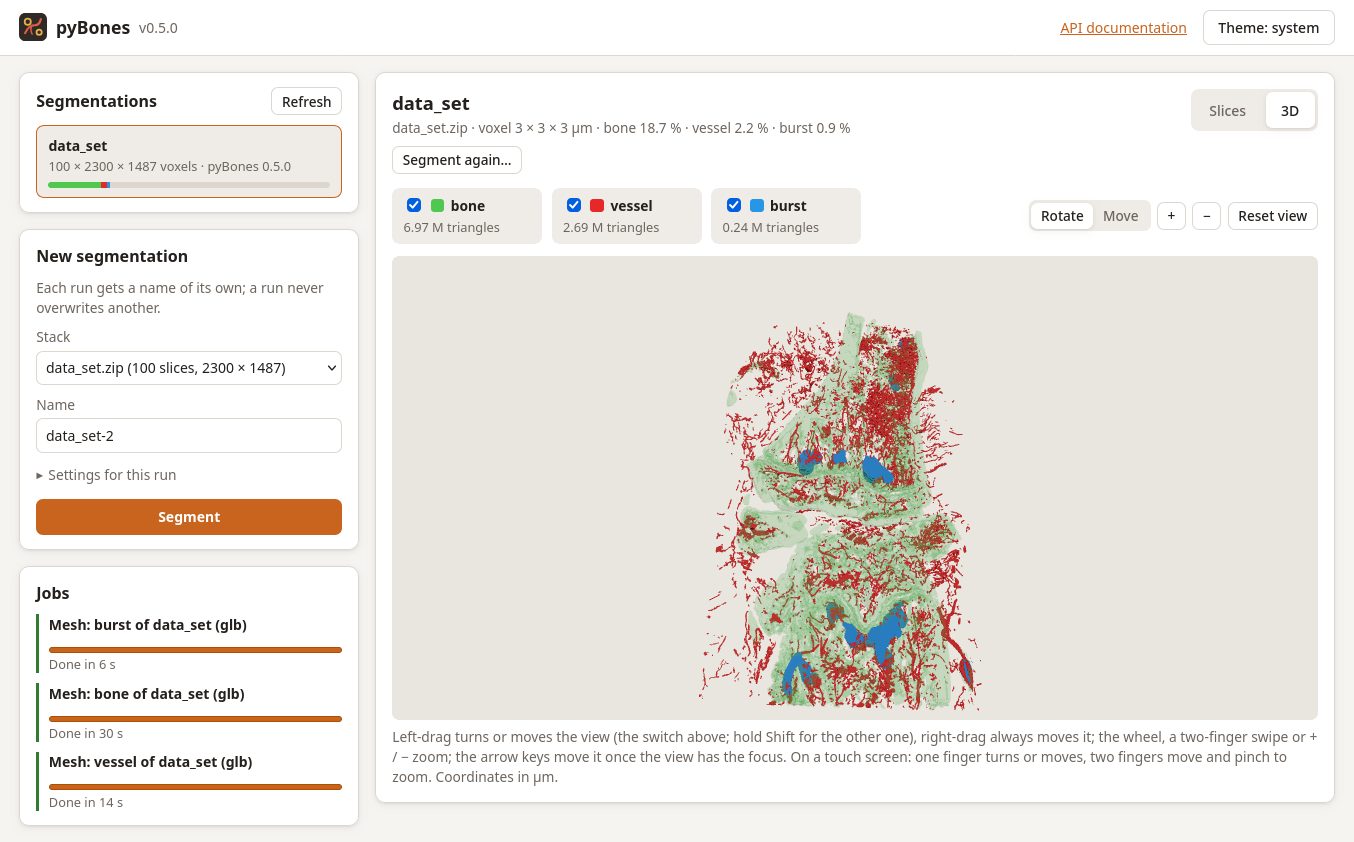
\includegraphics[width=\linewidth]{../../screenshots/06-web-page.png}
  \caption{The web page: segmentations and the jobs that built the meshes on the left; the meshes of
    the whole stack on the right, bone see-through, vessels in red, bursts in blue.}
  \label{fig:webpage}
\end{figure}

\begin{figure}[ht]
  \centering
  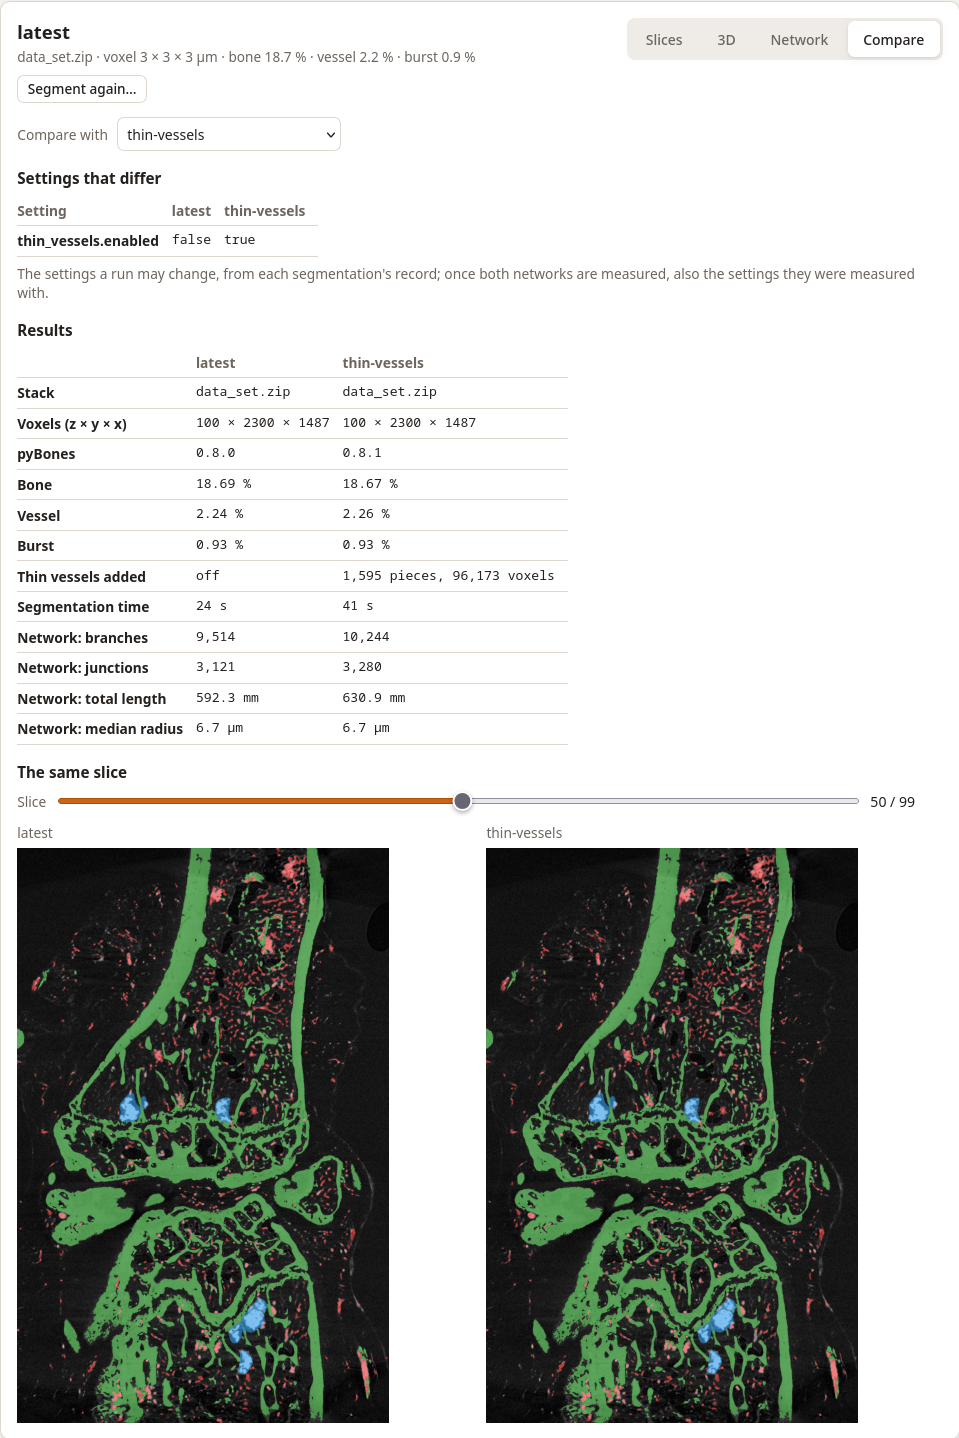
\includegraphics[width=0.75\linewidth]{../../screenshots/08-compare.png}
  \caption{The Compare tab: the sample segmented without and with the optional thin-vessel pass
    (Section~\ref{sec:thinvessels}): the setting that differs, the results side by side, and the
    same slice of both.}
  \label{fig:compare}
\end{figure}

\section{Pipeline}

\begin{figure}[ht]
\centering
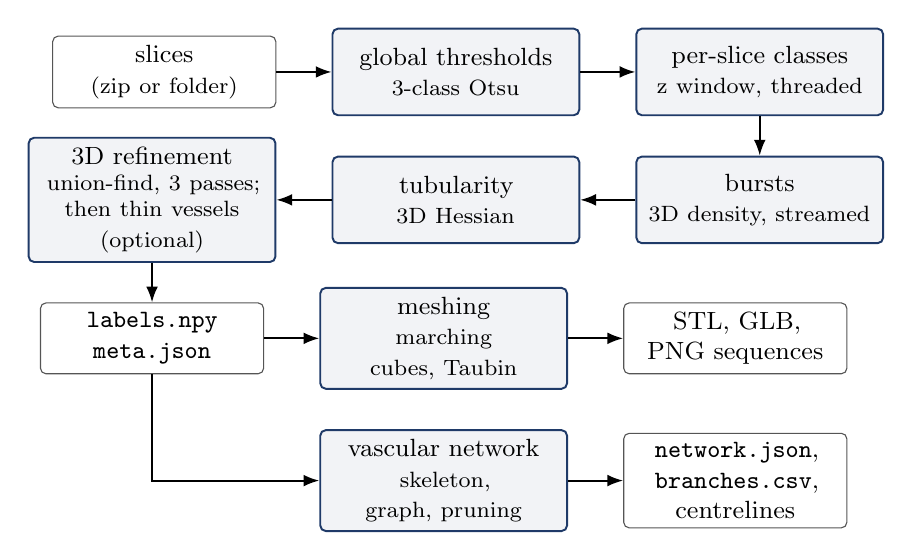
\begin{tikzpicture}[
  node distance=5mm and 7mm,
  box/.style={draw=accent,line width=0.7pt,rounded corners=2pt,fill=accent!6,align=center,
              minimum height=11mm,text width=29mm,font=\small},
  data/.style={draw=muted,rounded corners=2pt,fill=white,align=center,minimum height=9mm,
               text width=26mm,font=\small},
  arrow/.style={-{Latex[length=2mm]},line width=0.7pt,color=ink}]
  \node[data] (zip) {slices\\\footnotesize(zip or folder)};
  \node[box, right=of zip] (thr) {global thresholds\\\footnotesize 3-class Otsu};
  \node[box, right=of thr] (cls) {per-slice classes\\\footnotesize z window, threaded};
  \node[box, below=of cls] (burst) {bursts\\\footnotesize 3D density, streamed};
  \node[box, left=of burst] (tube) {tubularity\\\footnotesize 3D Hessian};
  \node[box, left=of tube] (ref) {3D refinement\\\footnotesize union-find, 3 passes;\\\footnotesize then thin vessels\\\footnotesize (optional)};
  \node[data, below=of ref] (vol) {\code{labels.npy}\\\code{meta.json}};
  \node[box, right=of vol] (mesh) {meshing\\\footnotesize marching cubes, Taubin};
  \node[data, right=of mesh] (stl) {STL, GLB,\\PNG sequences};
  \node[box, below=of mesh] (net) {vascular network\\\footnotesize skeleton, graph, pruning};
  \node[data, right=of net] (netfiles) {\code{network.json},\\\code{branches.csv}, centrelines};
  \draw[arrow] (zip) -- (thr);
  \draw[arrow] (thr) -- (cls);
  \draw[arrow] (cls) -- (burst);
  \draw[arrow] (burst) -- (tube);
  \draw[arrow] (tube) -- (ref);
  \draw[arrow] (ref) -- (vol);
  \draw[arrow] (vol) -- (mesh);
  \draw[arrow] (mesh) -- (stl);
  \draw[arrow] (vol) |- (net);
  \draw[arrow] (net) -- (netfiles);
\end{tikzpicture}
\caption{The pyBones pipeline. Only the boxes in the first two rows touch the raw data; each of them
  streams the stack slice by slice (or through a short window of slices).}
\label{fig:pipeline}
\end{figure}

\begin{enumerate}
  \item \textbf{Thresholds}: one 3-class Otsu for the whole stack (Section~\ref{sec:thresholds}).
  \item \textbf{Per-slice classification}: bright cores and their partial-volume rims are vessels,
        large bone-intensity regions are bone, small ones are marked \emph{ambiguous}
        (Section~\ref{sec:edges}).
  \item \textbf{Bursts}: dense clusters of bright pixels, measured per slice and in a 3D box
        (Section~\ref{sec:bursts}).
  \item \textbf{Tubularity}: a tube-versus-plate measure for every ambiguous voxel
        (Section~\ref{sec:tubularity}).
  \item \textbf{3D refinement}: each ambiguous 3D blob is decided by what it touches and by its shape;
        3D specks are removed (Section~\ref{sec:refinement}).
  \item \textbf{Thin vessels} (optional, off by default): thin pieces that a deconvolved image shows
        as bright as a vessel become vessel (Section~\ref{sec:thinvessels}).
  \item \textbf{Meshing}: surfaces for any label (Section~\ref{sec:meshing}).
  \item \textbf{Vascular network}: centrelines, a graph of branches and junctions, its measures
        (Chapter~\ref{chap:network}).
\end{enumerate}

\chapter{Segmentation, step by step}
\label{chap:segmentation}

This chapter follows the pipeline of Figure~\ref{fig:pipeline}. For each step: what the image
looks like, what the step does, and what it changed. I produced the ``before'' images by checking
out the corresponding past version of the code and running it on the same data
(Appendix~\ref{chap:reproduce}).

\section{One set of thresholds for the whole stack}
\label{sec:thresholds}

The three materials are visible as three modes of the intensity histogram
(Figure~\ref{fig:histogram}). A 3-class Otsu threshold maximises the between-class variance over every
pair of thresholds. pyBones runs it once, on the histogram of every fifth slice (after a light
Gaussian denoising), with an exhaustive search vectorised over a $1024 \times 1024$ grid of threshold
pairs. When the optimum is a plateau (an empty gap in the histogram), the centre of the plateau is
taken rather than its first element, which would sit on the tail of a class.

\begin{figure}[ht]
\centering
\begin{tikzpicture}
\begin{axis}[width=0.9\linewidth,height=5.2cm,ymode=log,xmin=0,xmax=45000,
  xlabel={intensity (16-bit grey level)},ylabel={fraction of voxels},
  tick label style={font=\small},label style={font=\small},
  scaled x ticks=false,xticklabel style={/pgf/number format/1000 sep={\,}}]
  \addplot[ink,thick] table[x=intensity,y=fraction,col sep=comma]{data/histogram.csv};
  \draw[accent,dashed,thick] (axis cs:\pbNumThrBone,1e-7) -- (axis cs:\pbNumThrBone,1);
  \draw[accent,dashed,thick] (axis cs:\pbNumThrVessel,1e-7) -- (axis cs:\pbNumThrVessel,1);
  \node[font=\footnotesize,anchor=south] at (axis cs:\pbNumMeanBackground,2e-2) {soft tissue};
  \node[font=\footnotesize,anchor=south,boneC!70!black] at (axis cs:\pbNumMeanBone,4e-3) {bone};
  \node[font=\footnotesize,anchor=south,vesselC] at (axis cs:\pbNumMeanVessel,1e-4) {contrast agent};
\end{axis}
\end{tikzpicture}
\caption{Histogram of the (smoothed) stack, log scale, with the two global thresholds
  (\pbValueThrBone{} and \pbValueThrVessel). The class means are \pbValueMeanBackground,
  \pbValueMeanBone{} and \pbValueMeanVessel.}
\label{fig:histogram}
\end{figure}

Per-slice thresholds, as in 2018, barely varied on this stack, but a single set guarantees that the
same tissue gets the same class everywhere, which every later 3D step relies on.

\section{Vessel edges at half-maximum}
\label{sec:edges}

\paragraph{The physics} A scanner blurs the image: every voxel averages the materials around it. A
voxel half filled with contrast agent and half with soft tissue reads halfway between the two
intensities; a voxel a quarter filled reads a quarter of the way. The natural boundary of a vessel is
therefore the \emph{half-maximum}: the voxels at least half filled with contrast agent. I measured the
blur of this scanner on the bone edges (the maximum gradient of a blurred step of contrast $C$
is $C / (\sigma\sqrt{2\pi})$): $\sigma \approx 1.45$ pixel, about 4.4\um.

\paragraph{The flaw it fixed} My first versions grew vessels from their bright cores down to a fixed
``weak'' threshold that sat at bone level. On the phantom (Chapter~\ref{chap:validation}) vessels came
out 1.75 times too thick, and a vessel lying against bone ate into it. Figure~\ref{fig:profile} shows
the effect on a real vessel: the 2018 mask and the 0.2 mask both extend well past the half-maximum.

\paragraph{The rule} For each candidate pixel near a bright core:
\[
  I \;\ge\; S + f\,(C - S),
\]
where $C$ is the brightest core within the rim radius (a grey-level dilation: the intensity of a fully
filled voxel of \emph{that} vessel, whatever its filling), $S$ the surrounding material, and
$f = 0.5$ the occupancy. The surround is read from the darkest intensity just beyond the rim (a
grey-level erosion): below the bone threshold it is soft tissue and the soft-tissue mean is used,
otherwise it is bone. A vessel running along bone is thus measured against bone and cannot eat into it.

Pixels near a core but below the half-maximum, with soft tissue around, form the \emph{halo}: a
vessel/soft-tissue mix whose intensity can reach bone level. They are background, not bone. This
replaced our 2018 rule, which turned every small blob holding a bright core into a vessel, halo
included.

\paragraph{In 3D} Cores and surround are searched in a 3D ball, not a disk. A vessel lying in the
slice plane blurs into the slices above and below; in those slices there is no bright core within
reach in 2D, so its blur used to become a ``bone collar'' around the vessel
(Figure~\ref{fig:collar}).

\begin{figure}[ht]
\centering
\begin{tikzpicture}
\begin{axis}[width=0.9\linewidth,height=5.6cm,xlabel={position across the vessel ($\mu$m)},
  ylabel={intensity},xmin=0,xmax=177,ymin=0,
  legend style={font=\footnotesize,at={(0.99,0.97)},anchor=north east,draw=none,fill=white,fill opacity=0.8},
  tick label style={font=\small},label style={font=\small},
  yticklabel style={/pgf/number format/1000 sep={\,}},scaled y ticks=false]
  \addplot[legacyC,only marks,mark size=1pt] table[x=x_um,y=raw,col sep=comma]{data/profile.csv};
  \addlegendentry{raw}
  \addplot[ink,thick] table[x=x_um,y=smoothed,col sep=comma]{data/profile.csv};
  \addlegendentry{smoothed}
  \draw[accent,dashed,thick] (axis cs:0,\pbNumProfileHalfMax) -- (axis cs:177,\pbNumProfileHalfMax);
  \node[accent,font=\footnotesize,anchor=south west] at (axis cs:2,\pbNumProfileHalfMax) {half-maximum};
  \addplot[legacyC,line width=4pt,unbounded coords=jump]
    table[x=x_um,y expr={\thisrow{legacy_vessel} > 0 ? 6000 : nan},col sep=comma]{data/profile.csv};
  \addlegendentry{2018 vessel mask}
  \addplot[vesselC!50,line width=4pt,unbounded coords=jump]
    table[x=x_um,y expr={\thisrow{v02_vessel} > 0 ? 3500 : nan},col sep=comma]{data/profile.csv};
  \addlegendentry{0.2 vessel mask}
  \addplot[vesselC,line width=4pt,unbounded coords=jump]
    table[x=x_um,y expr={\thisrow{current_vessel} > 0 ? 1000 : nan},col sep=comma]{data/profile.csv};
  \addlegendentry{\pbValueVersion{} vessel mask}
\end{axis}
\end{tikzpicture}
\caption{Intensity across a bright vessel (slice 0), and the extent of the vessel mask of each version
  (bars at the bottom). The half-maximum between the soft tissue and this vessel's core
  (\pbValueProfileCore) is \pbValueProfileHalfMax.}
\label{fig:profile}
\end{figure}

\begin{figure}[p]
\centering
\panel{0.24}{edges_vessels_raw.jpg}{Raw.}\hfill
\panel{0.24}{edges_vessels_v02.jpg}{0.2: fixed threshold.}\hfill
\panel{0.24}{edges_vessels_halfmax.jpg}{Half-maximum (2D).}\hfill
\panel{0.24}{edges_vessels_current.jpg}{\pbValueVersion: half-maximum in 3D.}
\caption{Marrow vessels. The fixed threshold of 0.2 draws the vessels wider than they appear; the
  half-maximum draws them at their visible width.}
\label{fig:edges}
\bigskip
\panel{0.24}{collar_raw.jpg}{Raw.}\hfill
\panel{0.24}{collar_halfmax.jpg}{Half-maximum (2D).}\hfill
\panel{0.24}{collar_tubes.jpg}{With the plate veto.}\hfill
\panel{0.24}{collar_current.jpg}{\pbValueVersion: 3D halo.}
\caption{A vessel lying in the slice plane, in soft tissue (lower vessel). Its blur in the neighbouring
  slices has no core within reach in 2D: first a vessel sheath, then (once plate-like blobs could not be
  vessels) a bone collar. Searching the cores in 3D removes most of it; a thin remnant remains on one
  side.}
\label{fig:collar}
\end{figure}

\section{Bursts}
\label{sec:bursts}

A burst is a cloud of contrast agent: a dense cluster of bright speckles, a few hundred micrometres
across (230 to 450\um{} on this scan). A thin vessel, even a bright one, is sparse at that scale.
I therefore measure the \emph{density} of bright pixels in a 123\um{} box around each pixel
(a box filter: integral-image speed), and declares a burst core where it exceeds 35\,\%.

\paragraph{In 3D} Measured per slice, the density flickers: near the top and bottom of a cluster a
slice only shows a sparse cross-section. Summing the per-slice densities over 41 slices (a running sum,
one addition and one subtraction per slice) gives the density in a 3D box, consistent along $z$. A cube
alone, however, erodes the ends of a cluster by up to half its depth: during development it lost a
whole cluster at slice 55. The final core is the union of the slice's own 2D core and the 3D core,
the latter only where the slice actually contains contrast agent (so a dense cluster cannot paint the
slices past its end). The density is stored on a 12\um{} grid, sixteen times smaller than per pixel,
since it is a mean over a much larger box.

\paragraph{The boundary} Our 2018 code and my early versions closed the core with a 45\um{} disk and
added an 18\um{} halo. On the phantom, I found every burst error 2 to 16 pixels on either side of the true
boundary: the radii imposed it. The boundary is now placed like the vessel edges, at a half-maximum: the
core grows over the pixels whose fine-scale density (36\um) stays above half the core density, then the
enclosed holes are filled (a purely topological operation, no radius).

\begin{figure}[ht]
\centering
\panel{0.24}{bursts_raw.jpg}{Raw (slice 55).}\hfill
\panel{0.24}{bursts_v02.jpg}{0.2: 2D density.}\hfill
\panel{0.24}{bursts_bursts3d.jpg}{3D density.}\hfill
\panel{0.24}{bursts_current.jpg}{\pbValueVersion: half-density edge.}
\caption{A burst cluster. Bursts are blue, vessels red.}
\label{fig:bursts}
\end{figure}

\begin{figure}[ht]
\centering
\begin{tikzpicture}
\begin{axis}[width=0.9\linewidth,height=5cm,xlabel={slice},ylabel={burst area (\% of the slice)},
  xmin=0,xmax=99,legend style={font=\footnotesize,at={(0.99,0.97)},anchor=north east,draw=none},
  tick label style={font=\small},label style={font=\small}]
  \addplot[legacyC,thick] table[x=z,y expr=100*\thisrow{v02},col sep=comma]{data/bursts_by_slice.csv};
  \addlegendentry{0.2 (2D density)}
  \addplot[burstC!60,thick] table[x=z,y expr=100*\thisrow{bursts3d},col sep=comma]{data/bursts_by_slice.csv};
  \addlegendentry{3D density}
  \addplot[burstC!80!black,thick] table[x=z,y expr=100*\thisrow{current},col sep=comma]{data/bursts_by_slice.csv};
  \addlegendentry{\pbValueVersion}
\end{axis}
\end{tikzpicture}
\caption{Burst area per slice on the real stack. A 3D object should change smoothly from one slice to
  the next; the 2D density makes it jump.}
\label{fig:bursts-z}
\end{figure}

\section{Ambiguous blobs and 3D connectivity}
\label{sec:refinement}

After the vessel edges and the bursts, the remaining bone-intensity regions are split by size: large
connected regions are bone, small ones (under 6300\umsq{} in the slice) are \emph{ambiguous}. A small
blob can be the cross-section of a trabecular rod, or a dim, clotted vessel: these are the ``zones of
uncertainty'' the researchers pointed out to us in 2018. In 3D the question has an answer: a rod joins the bone network, a
vessel joins vessels.

\paragraph{3D components without a 3D label volume} A 32-bit label volume of the stack would weigh
1.4\,GB. Instead, each slice is labelled in 2D (OpenCV), its labels are offset into a global numbering,
and labels of consecutive slices that touch (26-neighbourhood) are recorded as graph edges, looking only
at the previous slice. Since distinct 8-connected components of a slice never touch, the diagonal links
only need to be checked on the thin band where the voxel straight below is background; this cut the
time of the whole refinement by almost three in my measurements. The graph is solved once by a vectorised union-find (every root hooks onto its
smallest neighbouring root, then pointer jumping flattens the forest, until no edge spans two trees).
Any slice can later be re-labelled and mapped through the result, so at most two label slices are ever
in memory.

\paragraph{The decision} Each ambiguous 3D component is decided in three streamed passes:
\begin{itemize}
  \item small and isolated: noise, background;
  \item plate-like (Section~\ref{sec:tubularity}): never a vessel; bone if it touches bone,
        background otherwise (the sheath of a vessel, a fascia);
  \item otherwise \vessel{} if it touches vessels more than bone, or if it is isolated (bone cannot
        float), \bone{} if it touches bone.
\end{itemize}
Finally, vessel and bone 3D components smaller than a minimum volume are removed. I kept our 2018
three-slice majority vote available but disabled it: once 3D connectivity exists, it only fragmented the
bone network (783 bone components instead of 45) for no gain.

\section{Tubes versus plates}
\label{sec:tubularity}

The curvature of the intensity tells shapes apart. At each voxel, the Hessian matrix (second
derivatives) has three eigenvalues $|\lambda_1| \le |\lambda_2| \le |\lambda_3|$: a bright tube curves
strongly in two directions ($\lambda_2 \approx \lambda_3 \ll 0$, $\lambda_1 \approx 0$), a bright plate in
one ($\lambda_3 \ll 0$, $\lambda_1 \approx \lambda_2 \approx 0$), a blob in three. The ratio
$R_A = |\lambda_2| / |\lambda_3|$ is close to 1 for a tube and to 0 for a plate, whatever the contrast.

The Hessian is computed at three scales (3, 4.5 and 6\um) from Gaussian derivatives, streamed through
a window of 13 slices: the raw slices are first combined along $z$ with the three derivative kernels,
then filtered in-plane, never storing a volume. The eigenvalues of millions of $3 \times 3$ symmetric
matrices are computed in closed form (Smith's trigonometric formula), in chunks, only on the voxels that
can become ambiguous.

\paragraph{What it can and cannot do} I tried Frangi's classic vesselness filter first. On the phantom
it separated vessels from bone pieces only through contrast; on shape alone it did no better than
chance: trabecular rods \emph{are} tubes. Plates, however, are separated very well: the mean $R_A$ of
an ambiguous component distinguished true vessels from bone pieces with an area under the ROC curve of
0.93. I therefore use $R_A$ for one thing only, a veto: a component whose mean ratio is below
0.45 cannot be a vessel (Figure~\ref{fig:tubularity}). On the phantom it corrected the largest
misclassified bone fragments (two of them 6\,000 and 17\,000 voxels) without losing any true vessel.

\begin{figure}[ht]
\centering
\panel{0.4}{tubularity_raw.jpg}{Raw (slice 50, marrow).}\hspace{0.05\linewidth}
\panel{0.4}{tubularity_map.jpg}{Mean tube-vs-plate ratio per blob.}
\caption{Ambiguous blobs coloured by their mean ratio $R_A$: blue blobs are plate-like (vetoed),
  green to red ones tube-like. The 3D decision uses the mean over each 3D component; this is its 2D view.}
\label{fig:tubularity}
\end{figure}

\section{Meshing}
\label{sec:meshing}

Surfaces are extracted per label with marching cubes (scikit-image, the only use of that library).
The label volume is first downsampled by an exact block mean, which keeps sub-voxel information and
divides the memory by $8$ (factor 2). Marching cubes on voxel data produces ``staircase'' surfaces
(the ``cubic aspect'' noted in 2018): on a voxelised sphere the surface area is 8.5\,\% too large.
Taubin's $\lambda|\mu$ smoothing alternates a shrinking and an inflating step, which removes the
staircase without shrinking the object: the area error falls to 0.8\,\% in 10 iterations, the volume
is kept, and a two-voxel-thin tube keeps 92\,\% of its volume (blurring the volume before meshing would
erase it).

Meshes are written in micrometres, in one of two formats. Binary STL, for other software, stores every
triangle with its own three corners as 32-bit floats. Binary glTF (GLB), for the browser, stores each
point once and the triangles as indices into them, and can store the positions as 16-bit integers over
the mesh's bounding box (the \code{KHR\_mesh\_quantization} extension), with 8-bit normals. A point is
then off by at most half of the box size divided by 65\,535 on each axis: 0.05\um{} on the sample,
sixty times less than a voxel. Table~\ref{tab:meshfiles} compares the three choices on the vessel mesh
of the sample. The storage precision is not the grid the surface is built on: with the default factor
of 2, that grid is 6\um{}.

\begin{table}[ht]
\centering
\small
\begin{tabular}{@{}lrll@{}}
\toprule
Format          & Size          & Position error              & Use \\
\midrule
STL             & 134.6\,MB     & none (32-bit floats)        & other software (ImageJ, MeshLab) \\
GLB, 32-bit     & 64.7\,MB      & none (32-bit floats)        & browser, exact positions \\
GLB, 16-bit     & 48.5\,MB      & $\leq 0.05$\um{}            & browser (default) \\
\bottomrule
\end{tabular}
\caption{The vessel mesh of the sample (1.35 million points, 2.7 million triangles, 6\um{} grid) in
each file format.}
\label{tab:meshfiles}
\end{table}

Figure~\ref{fig:network} shows the vessel network of the whole stack, viewed from above.

\begin{figure}[ht]
\centering
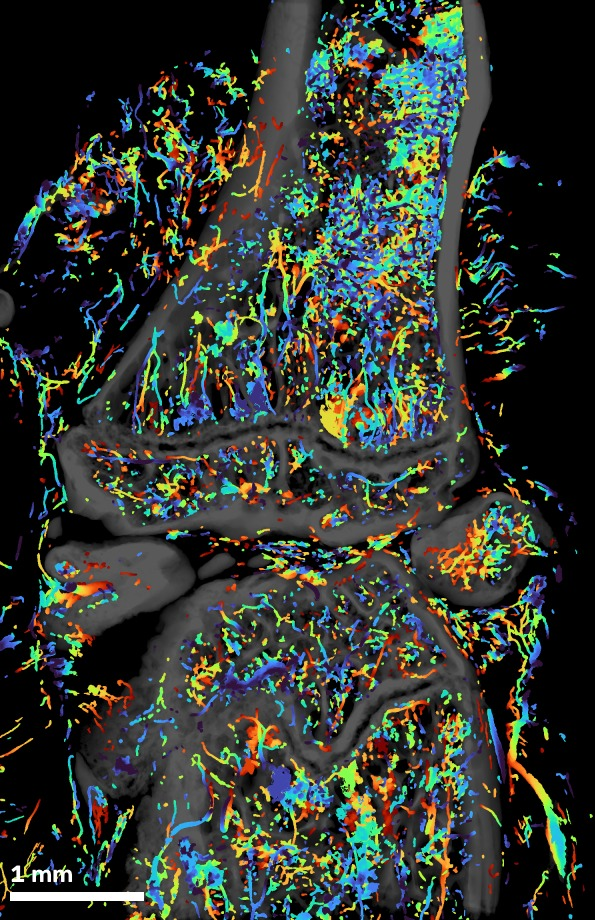
\includegraphics[width=0.62\linewidth]{vessel_network.jpg}
\caption{The vessels of the whole stack seen from above, coloured by depth (blue: first slices, red:
  last slices), over a faint projection of the bone. Marrow vessels of the femur (top) and tibia
  (bottom), and the soft-tissue vessels around the joint.}
\label{fig:network}
\end{figure}

\chapter{Validation}
\label{chap:validation}

\section{No ground truth}

To improve a segmentation, I had to be able to tell that it improved. Our 2018 masks are not a ground
truth: they encode our 2018 method, fat vessels included (Figure~\ref{fig:profile}). Expert annotation
is the usual answer, but none is available for this scan: I am no longer in touch with the researchers,
and annotating these images requires an expertise I do not have. Labels I painted myself would only
encode the algorithm's own assumptions.

I built two tools to address this. The first is ready for whoever can provide expert labels; the second
is the metric I actually used.

\paragraph{An annotation page} \code{tools/annotation} picks about ten crops of 256 pixels from a
segmentation (burst-rich, vessel-rich and random tissue), each with three slices of context on either
side, and serves a local web page (standard-library server, no extra dependency) to paint them
(Figure~\ref{fig:annotation}): brush, bucket fill, a ``wand'' that fills the connected pixels of
similar brightness (a click inside a vessel stops at its edge), undo, and an \emph{unsure} label excluded
from the scores. The view can be zoomed, panned and re-contrasted, the labels shown as outlines only,
the brush restricted to pixels of one label (to paint a vessel against bone without touching the bone),
and each crop carries a free-text note for doubts. Work is saved automatically. Crops can start from the current segmentation (much faster, but biased toward the algorithm,
which the manifest records). A \code{score} command then reports per-class agreement and the
confusion matrix against any segmentation.

\begin{figure}[ht]
  \centering
  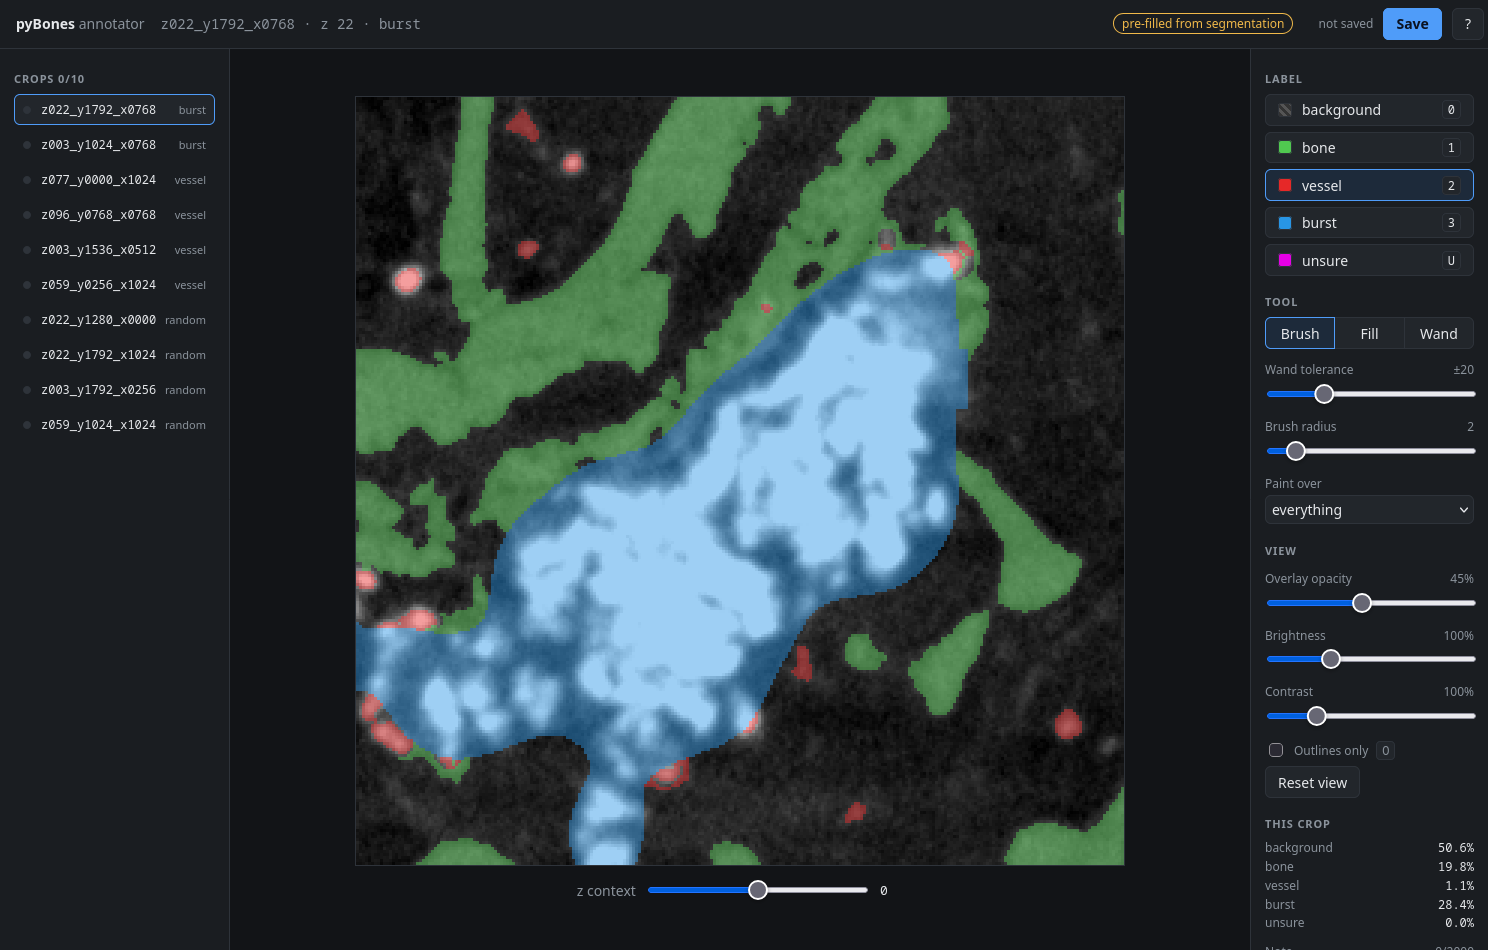
\includegraphics[width=0.85\linewidth]{../../screenshots/05-annotation-tool.png}
  \caption{The annotation page: crops on the left, the label palette and tools on the right; the
    arrow keys browse the neighbouring slices, the way a vessel is told from a trabecula by eye.}
  \label{fig:annotation}
\end{figure}

\section{A synthetic phantom}

\code{tools/phantom} renders a $\mu$CT-like volume ($96 \times 512 \times 512$ voxels of 3\um) whose
labels are known exactly:
\begin{itemize}
  \item cortex walls and trabecular plates (discs), and trabecular rods \emph{bridging} two plates;
  \item vessels as smooth random walks of tube segments of 3 to 25\um{} radius, some segments clotted
        (20 to 50\,\% filled), some empty (invisible, excluded from the scores);
  \item burst clusters: spheres of 110 to 200\um{} radius filled with dense speckles and a diffuse haze;
  \item every shape rendered with a partial-volume edge, then blurred and corrupted by noise.
\end{itemize}
Its parameters are calibrated on the real scan: the class intensities (medians of each class), the noise
(and its growth with intensity), the burst sizes, and the blur, measured on the real bone edges
($\sigma = 4.4$\um). A score reports, per class, the Dice coefficient (overlap), the precision (how much
of what was labelled is right) and the recall (how much of the truth was found), plus the vessel recall
per radius band and on clotted segments.

A phantom only helps if it is realistic, and mine was wrong twice during development. First, its rods
floated freely: the rule ``bone cannot float'' then labelled them as vessels, which no real rod does.
Second, its bursts were half the size of the real ones, below the detector's minimum area: the phantom
was unfair to the algorithm. I fixed both by measuring the real data (rod geometry, burst sizes)
before trusting a score again.

\begin{figure}[ht]
\centering
\panel{0.32}{phantom_raw.jpg}{Phantom slice.}\hfill
\panel{0.32}{phantom_truth.jpg}{Exact ground truth.}\hfill
\panel{0.32}{phantom_segmentation.jpg}{Segmentation (\pbValueVersion).}
\caption{A slice of the phantom. Today's scores: bone Dice \pbValueBoneDice, vessel Dice
  \pbValueVesselDice{} (precision \pbValueVesselPrecision, recall \pbValueVesselRecall), burst Dice
  \pbValueBurstDice; \pbValueAccuracy{} of all voxels correct.}
\label{fig:phantom}
\end{figure}

\section{Every version, on the same ground truth}

I recorded each milestone of the rewrite as a commit of my development repository.
\code{python -m tools.report history} checks each of them out in its own git worktree, with its own
environment, runs it on the \emph{current} phantom and scores it with today's scorer. The comparison
is therefore fair: same input, same metric, only the code changes (Table~\ref{tab:history},
Figure~\ref{fig:history}). The published repository starts from the final state and does not hold
those commits: their scores and the few slices the figures show are kept as an archive
(\code{docs/report/data/}), and only the current version is run again.

\begin{table}[ht]
\centering
\small
\begin{tabular}{@{}l l r r r r r r@{}}
\toprule
Version & Commit & Bone & Vessel & (prec.) & (recall) & Burst & Real stack \\
\midrule
First Python port (2D, per-slice) & \texttt{6e040e7} & 0.972 & \textbf{0.709} & 0.569 & 0.943 & 0.887 & 4\,s / 0.3\,GB \\
3D connectivity refinement & \texttt{3d05cea} & 0.975 & \textbf{0.674} & 0.521 & 0.953 & 0.884 & 12\,s / 0.8\,GB \\
3D burst density & \texttt{222b1a4} & 0.975 & \textbf{0.686} & 0.536 & 0.953 & 0.897 & 12\,s / 1.2\,GB \\
Physical units, analytic kernels & \texttt{fe645dd} & 0.974 & \textbf{0.685} & 0.535 & 0.954 & 0.897 & -- \\
Half-maximum vessel edges & \texttt{50a394c} & 0.986 & \textbf{0.810} & 0.719 & 0.928 & 0.897 & 12\,s / 1.3\,GB \\
Tube-vs-plate veto & \texttt{427cd3d} & 0.989 & \textbf{0.829} & 0.753 & 0.923 & 0.897 & 33\,s / 3.0\,GB \\
3D vessel halo & \texttt{e7ca4a1} & 0.989 & \textbf{0.837} & 0.776 & 0.907 & 0.897 & -- \\
Half-maximum burst boundary & \texttt{d33da52} & 0.989 & \textbf{0.840} & 0.801 & 0.884 & 0.911 & -- \\
Current code (0.7.0) & -- & 0.989 & \textbf{0.862} & 0.826 & 0.901 & 0.922 & 24\,s / 1.7\,GB \\
\bottomrule
\end{tabular}

\caption{Dice score per class on the phantom for every milestone of the rewrite, vessel precision and
  recall, and the cost of segmenting the real stack (wall time and peak memory, all measured on the
  machine described in Chapter~\ref{chap:performance}; ``--'' when that version was not run on the real
  data).}
\label{tab:history}
\end{table}

\begin{figure}[ht]
\centering
\begin{tikzpicture}
\begin{axis}[width=0.95\linewidth,height=6cm,ymin=0.6,ymax=1.0,ylabel={Dice},
  xtick=data,xticklabels from table={\historytable}{key},
  xticklabel style={rotate=35,anchor=east,font=\footnotesize\ttfamily},
  legend style={font=\footnotesize,at={(0.5,-0.38)},anchor=north,legend columns=3,draw=none},
  tick label style={font=\small},label style={font=\small},grid=major,grid style={muted!20}]
  \addplot[boneC!70!black,thick,mark=*] table[x expr=\coordindex,y=bone_dice]{\historytable};
  \addlegendentry{bone}
  \addplot[vesselC,thick,mark=*] table[x expr=\coordindex,y=vessel_dice]{\historytable};
  \addlegendentry{vessel}
  \addplot[burstC,thick,mark=*] table[x expr=\coordindex,y=burst_dice]{\historytable};
  \addlegendentry{burst}
\end{axis}
\end{tikzpicture}
\caption{Dice per class along the history of the rewrite (same phantom, same scorer).}
\label{fig:history}
\end{figure}

I read the history as follows.
\begin{itemize}
  \item The \textbf{first port} (0.1, close in spirit to 2018 but with global thresholds and labelled
        bursts) already finds most vessels (high recall) but labels far too much as vessel (precision
        about 0.57): the vessels are fat.
  \item The \textbf{3D refinement} of 0.2 \emph{lowered} the vessel score at first, which surprised me. It turned many
        ambiguous blobs into vessels, which was right in spirit but only added more voxels to vessels
        that were already too thick. A better decision rule cannot fix wrong edges.
  \item The \textbf{half-maximum edges} are the turning point: the largest single gain of the rewrite,
        on vessels and on bone alike. Physics beat parameter tuning.
  \item The \textbf{plate veto}, the \textbf{3D halo} and the \textbf{burst boundary} each add a
        smaller, measured gain. Today's version measures that boundary in 3D: bursts no longer follow
        and hollow out the vessels lying in a slice (Section~\ref{sec:bursts}), which raises both the
        vessel and the burst scores; earlier, it had become faster and lighter (tubularity computed
        only where it is used).
\end{itemize}

\begin{figure}[ht]
\centering
\begin{tikzpicture}
\begin{axis}[width=0.95\linewidth,height=5.5cm,ymin=0,ymax=1.0,ylabel={vessel recall},
  xtick=data,xticklabels from table={\historytable}{key},
  xticklabel style={rotate=35,anchor=east,font=\footnotesize\ttfamily},
  legend style={font=\footnotesize,at={(0.5,-0.38)},anchor=north,legend columns=4,draw=none},
  tick label style={font=\small},label style={font=\small},grid=major,grid style={muted!20}]
  \addplot[vesselC!40,thick,mark=*] table[x expr=\coordindex,y=vessel_recall_0_6um]{\historytable};
  \addlegendentry{radius 0--6\um}
  \addplot[vesselC!70,thick,mark=*] table[x expr=\coordindex,y=vessel_recall_6_12um]{\historytable};
  \addlegendentry{radius 6--12\um}
  \addplot[vesselC,thick,mark=*] table[x expr=\coordindex,y=vessel_recall_12_25um]{\historytable};
  \addlegendentry{radius 12--25\um}
  \addplot[ink,thick,dashed,mark=o] table[x expr=\coordindex,y=clotted_recall]{\historytable};
  \addlegendentry{clotted segments}
\end{axis}
\end{tikzpicture}
\caption{Vessel recall per radius band and on clotted segments. Thin vessels are found far less often
  than large ones (Section~\ref{sec:thin}); the recall of large vessels decreases slightly as their
  edges become exact (fat masks ``find'' every truth voxel).}
\label{fig:history-recall}
\end{figure}

\section{On the real scan}

Figure~\ref{fig:real-overview} compares the 2018 masks with today's segmentation on a whole slice, and
Figure~\ref{fig:real-evolution} follows one region through the versions. Today, the stack is
\pbValueFracBone\,\% bone, \pbValueFracVessel\,\% vessel and \pbValueFracBurst\,\% burst.

\begin{figure}[ht]
\centering
\panel{0.4}{overview_legacy.jpg}{2018 masks (bone, vessels; bursts were discarded).}\hspace{0.05\linewidth}
\panel{0.4}{overview_current.jpg}{Version \pbValueVersion{} (bone, vessels, bursts).}
\caption{Slice 0, the 2018 segmentation and today's.}
\label{fig:real-overview}
\end{figure}

\begin{figure}[p]
\centering
\panel{0.32}{evolution_marrow_raw.jpg}{Raw.}\hfill
\panel{0.32}{evolution_marrow_legacy.jpg}{2018 (Matlab).}\hfill
\panel{0.32}{evolution_marrow_v01.jpg}{0.1: first port.}\\[6pt]
\panel{0.32}{evolution_marrow_v02.jpg}{0.2: 3D refinement.}\hfill
\panel{0.32}{evolution_marrow_halfmax.jpg}{Half-maximum edges.}\hfill
\panel{0.32}{evolution_marrow_current.jpg}{\pbValueVersion.}
\caption{One marrow region through the versions. 2018: fat vessels, bursts left unlabelled. 0.1: bursts
  found, but thin dim vessels lost to bone. 0.2: vessels back, still fat and wrapped in bone. Half-maximum
  edges and the later steps: vessels at their visible width, trabeculae untouched.}
\label{fig:real-evolution}
\end{figure}

\chapter{Speed and memory}
\label{chap:performance}

I treated speed and memory as constraints from the start, but never at the expense of correctness:
each optimisation came after the result it served was right, and I checked that it left the output
unchanged (byte-identical, or with every difference explained). Today the whole stack is segmented in
about \pbValueSeconds\,s with a peak of \pbValuePeakGB\,GB of memory.

\paragraph{Test machine} Timings depend on the hardware, so they are only meaningful next to it. Every
timing of this report (here and in Table~\ref{tab:history}) was measured on the same machine, recorded
automatically when the runs were timed:
\begin{center}
\small
\begin{tabular}{@{}ll@{}}
\toprule
Processor        & \pbValueCpu{} (\pbValueCores{} logical cores) \\
Memory           & \pbValueMemoryGB\,GB \\
System           & \pbValueSystem \\
Python           & \pbValuePython{} (report tool) \\
pyBones threads  & \pbValueWorkers{} (\code{pipeline.workers}) \\
\bottomrule
\end{tabular}
\end{center}
The times are wall-clock times of the whole command, including the start-up of each version's
environment; the memory is the peak resident size of the process tree. On another machine the absolute
values will differ; the comparison between versions holds, since they all ran on this one.

\paragraph{What makes it fast}
\begin{itemize}
  \item \textbf{Vectorisation}: no Python loop ever runs over pixels or labels. Component statistics are
        one \code{bincount}, morphological reconstruction one labelling, the Otsu search one array
        expression over all threshold pairs, the eigenvalues a closed formula over millions of matrices.
  \item \textbf{OpenCV} for every filter: Gaussian blurs, box filters (integral images), grey-level
        dilations and erosions, connected components, separable Hessian filters.
  \item \textbf{Threads} for the per-slice work (about twice as fast with four threads).
  \item \textbf{Work only where it matters}: the Hessian eigenvalues are computed only on the voxels that
        can become ambiguous, a few percent of each slice instead of a quarter of it.
\end{itemize}

\paragraph{What keeps memory low}
\begin{itemize}
  \item \textbf{Streaming}: slices go through bounded windows; volumes are written slice by slice and
        read back memory-mapped. A full 32-bit label volume (1.4\,GB) or six float Hessian volumes
        (8\,GB) are never built.
  \item \textbf{Compact buffers}: the slices waiting for the 3D burst box are bit-packed (eight times
        smaller), the burst density lives on a 12\um{} grid (sixteen times smaller), the tubularity is
        stored on one byte.
  \item \textbf{Chunks}: eigenvalues, mesh smoothing, normals and mesh writing process bounded
        batches.
\end{itemize}

\paragraph{Meshes} Extracting and smoothing the surface of the vessels takes
\pbValueMeshVesselSeconds\,s and that of the bone \pbValueMeshBoneSeconds\,s on the same machine, most
of it in the Taubin smoothing; writing the file adds a few seconds. A mesh job reports
four weighted stages (block occupancy, surface, smoothing, file), so its progress bar moves with the
work, and it can be cancelled between them.

\paragraph{On the web page} A page that stays open for hours must not grow: an image cache that never
empties is enough to crash a browser. So the page holds every resource once:
\begin{itemize}
  \item \textbf{Slices are never kept.} Each one is fetched with the browser's cache disabled, shown
        through a temporary \code{blob:} address that is released as soon as the image is decoded, and
        the server forbids caching it as well. Scrolling through a stack for hours costs one image.
  \item \textbf{One slice request at a time.} Dragging the slider never piles renders up on the
        server: a position asked for during a render waits, and only the latest one is fetched.
  \item \textbf{Meshes live on the graphics card.} The CPU copy that three.js keeps after uploading a
        mesh is released, which halves the browser's share; a segmentation left behind frees its
        meshes. A mesh may be kept by the browser between visits, but it is checked each time, so a
        rebuilt mesh is never hidden by an old copy.
  \item \textbf{Following a job holds no thread.} Job events reach the browser through the server's
        event loop, so any number of open pages cannot starve the slice and list requests.
\end{itemize}

My last optimisation pass brought the segmentation from 36\,s and 3.3\,GB to the figures above, and the
smoothing of the bone mesh (about 7 million triangles) from 1.9\,GB to 1.2\,GB with an identical result.
Version 0.1 was faster and lighter still, but it computed much less: the 3D refinement and the
tubularity are what the time and memory now buy.

\chapter{Current limitations}
\label{chap:limitations}

\section{Thin vessels are below the resolution}
\label{sec:thin}

With a blur of $\sigma = 4.4$\um{}, the image of a point is about 10\um{} wide at half its height. A
vessel of 3 to 6\um{} radius is narrower than the blur: its image is essentially the blur's own shape,
dimmer than a large vessel, whatever its true size. On the phantom, vessels of that size are found
\pbValueVesselRecallThin{} of the time, against \pbValueVesselRecallMedium{} for 6--12\um{} and
\pbValueVesselRecallLarge{} above.

I tried two recoveries and dropped them. The missed thin vessels turned out not to be faint at all (their
voxels are mostly brighter than the bone threshold): they are lost because, next to a brighter vessel,
they fall below that vessel's half-maximum and are taken for its halo. Telling them apart from a real
halo with the Hessian recovered about as many wrong voxels as right ones: no net gain, so I did not
keep the code. The
consequence for future measurements is that diameters under about 12\um{} will be overestimated, and
the thinnest vessels partly missed: this is a property of the scan, not of the software.

\section{Rods and vessels}

Shape alone cannot tell a trabecular rod from a vessel: both are tubes. The decision rests on what they
touch in 3D. A dim vessel running along a trabecula, or a rod touching vessels on all sides, can still
be misclassified; these are the same ``zones of uncertainty'' we met in 2018.

\section{Validation}

The phantom is calibrated on the real scan, but it is synthetic: its vessel paths, burst textures and
bone geometry are simplifications. The scores of Chapter~\ref{chap:validation} measure the method on
realistic data, not the segmentation of this particular knee. Expert labels on a few real crops (the
annotation page is ready) would close that gap.

\section{The data}

\begin{itemize}
  \item \textbf{One sample.} I could only check the parameters on a single scan. Physical units make them
        transferable in principle, not in fact.
  \item \textbf{Voxel size.} 3\um{} is the slice thickness we used in 2018 and agrees with the
        anatomy; I assumed isotropy.
  \item \textbf{A thin slab.} The stack is 100 slices thick (0.3\,mm) for a knee several millimetres
        wide: most vessels leave the volume, which limits what 3D connectivity can decide near the
        first and last slices.
  \item \textbf{Bursts and vessels.} A vessel running into a burst cluster is partly absorbed by it.
\end{itemize}

\section{The original goal}

The brief asked for a quantified network: nodes, branches, calibre, branch lengths. pyBones delivers a
validated segmentation and meshes, the prerequisite, but not the quantification yet.

\chapter{Conclusion}
\label{chap:conclusion}

In 2018, the four of us built, in a few weeks, a segmentation that the researchers approved, and a
viewer for it. We had identified the real difficulty, telling vessels from bone, and answered it with
morphology tuned by eye.

Eight years later, pyBones keeps the goal and changes the method. The main lessons I draw from the
rewrite are:
\begin{itemize}
  \item \textbf{Measure before improving.} Without a ground truth, a synthetic phantom calibrated on the
        real scan made every change measurable, and showed me that an intuitive improvement (the first 3D
        refinement) made things worse until the vessel edges were right.
  \item \textbf{Physics over parameters.} The largest gains came from modelling how the image forms
        (partial volume, blur, density) rather than from tuning radii: half-maximum edges for vessels
        and bursts, physical units for every size.
  \item \textbf{3D where 2D cannot decide.} Connectivity and shape in 3D resolve most of the blobs that a
        single slice leaves ambiguous; what remains is a property of the scan (resolution) and of the
        anatomy (rods are tubes too).
\end{itemize}

\section*{Future work}
\addcontentsline{toc}{section}{Future work}

\begin{itemize}
  \item \textbf{Quantification}, the original goal: vessel centrelines, network graph, node and branch
        counts, calibre (with the resolution caveat of Section~\ref{sec:thin}) and branch lengths.
  \item \textbf{Gap bridging} along the vessel direction, to reconnect vessels interrupted by clots.
  \item \textbf{Expert validation} of a few real crops with the annotation page.
  \item \textbf{A web page} on top of the web server: slices with their labels, and an in-browser 3D
        view of lighter meshes.
\end{itemize}


\appendix
\chapter{Reproducing this report}
\label{chap:reproduce}

Everything below runs from the repository root, with the dataset saved as
\code{data/data\_set.zip}, and needs uv and git. How to install the project from scratch is in
\code{INSTALL.md}; the report's steps, in more detail, are in \code{CONTRIBUTING.md}.

\begin{enumerate}
  \item Generate the phantom (the stack itself is segmented by the next step):
\begin{verbatim}
uv run python -m tools.phantom generate -o output/phantom
\end{verbatim}
  \item Run every version listed in \code{tools/report/config.json} on the phantom (and on the real
        data where figures need it), each in its own git worktree and environment, and score them:
\begin{verbatim}
uv run python -m tools.report history
\end{verbatim}
        This writes \code{docs/report/data/history.csv} and, for each version, a small extract of its
        segmentation (\code{docs/report/data/runs/}). Versions whose commit is not in the repository
        are not run again: their archived scores and extracts are kept. Each run records the machine
        and the power profile it ran on; timings are only comparable when every version ran in one
        session, under one profile, with nothing else running (Chapter~\ref{chap:performance}).
  \item Render the figures, the plot data, the history table, the mesh measurements (each label
        meshed and written in every format), the vascular network of Chapter~\ref{chap:network} (the
        sample measured, the branching phantom generated, segmented and scored afresh), the two
        experimental switches on both phantoms and the sample (Section~\ref{sec:experimental}), and
        the measured values (\code{values.tex}), the stage weights of the progress bars, and the README's
        tables and first screenshots; about four minutes:
\begin{verbatim}
uv run python -m tools.report figures
\end{verbatim}
  \item Build the PDF (XeLaTeX; settings in \code{docs/report/latexmkrc}):
\begin{verbatim}
cd docs/report && latexmk report.tex
\end{verbatim}
\end{enumerate}

The 2018 images of Chapter~\ref{chap:legacy} and the 2018 masks used for the comparisons are stored
in \code{docs/report/2018/}.
The screenshots of the annotation page and of the web page were taken from the running pages in a
browser; the report tool does not produce them.


\end{document}
